\begin{frame}
    \frametitle{Best Performing Transition Scenarios}
    \textbf{Input Parameters of best performing transition scenarios}
    \begin{table}[]
        \resizebox{\textwidth}{!}{%
        \begin{tabular}{|l|l|c|l|l|l|}
        \hline
        \multirow{2}{*}{}                         & \multicolumn{1}{c|}{\multirow{2}{*}{\textbf{Input Parameter}}} & \multicolumn{4}{c|}{\textbf{Simulation Description}}                                                                                                                                                                                                                                                       \\ \cline{3-6} 
                                                  & \multicolumn{1}{c|}{}                                          & \multicolumn{1}{l|}{\textbf{EG01-23}}                                                                 & \textbf{EG01-24}                  & \textbf{EG01-29}                 &\textbf{EG01-30}                                                  \\ \hline
        \multirow{4}{*}{\textbf{Required}} & Demand driving commodity                                       & \multicolumn{4}{c|}{Power}                                                                                                                                                                                                                                                                                 \\ \cline{2-6} 
                                                  & Demand equation [MW]                                               & \multicolumn{1}{l|}{60000}                                                                                & $60000 + 250t/12$ & 60000                     &     $60000 + 250t/12$                                       \\ \cline{2-6} 
                                                  & Prediction method                                              & \texttt{poly}       & \texttt{fft}             & \texttt{poly}         &  \texttt{fft}    \\ \cline{2-6} 
                                                  & Deployment Driving Method                                      & \multicolumn{4}{c|}{Installed Capacity}                                                                                                                                                                                                                                                                    \\ \hline
        \multirow{2}{*}{\textbf{Optional}} & Buffer type                                                    & \multicolumn{4}{c|}{Absolute}                                                                                                                                                                                                                                                               \\ \cline{2-6} 
                                                  & Power Buffer size [MW]                                                   & 0 & 6000 & 0 & 8000 \\ \hline
        \end{tabular}%
        }
        \caption{\deploy's input parameters for EG01-EG23, EG01-EG24, EG01-EG29, and 
        EG01-EG30 transition scenarios
        that minimizes undersupply of power and minimizes 
        the undersupply and under capacity of the other facilities. }
        \label{tab:bestinputs}
        \end{table}
\end{frame}

\begin{frame}
    \frametitle{Best Performing Transition Scenarios}
    \textbf{EG01-23: Constant Power Demand}
    \begin{figure}[htbp!]
        \begin{center}
          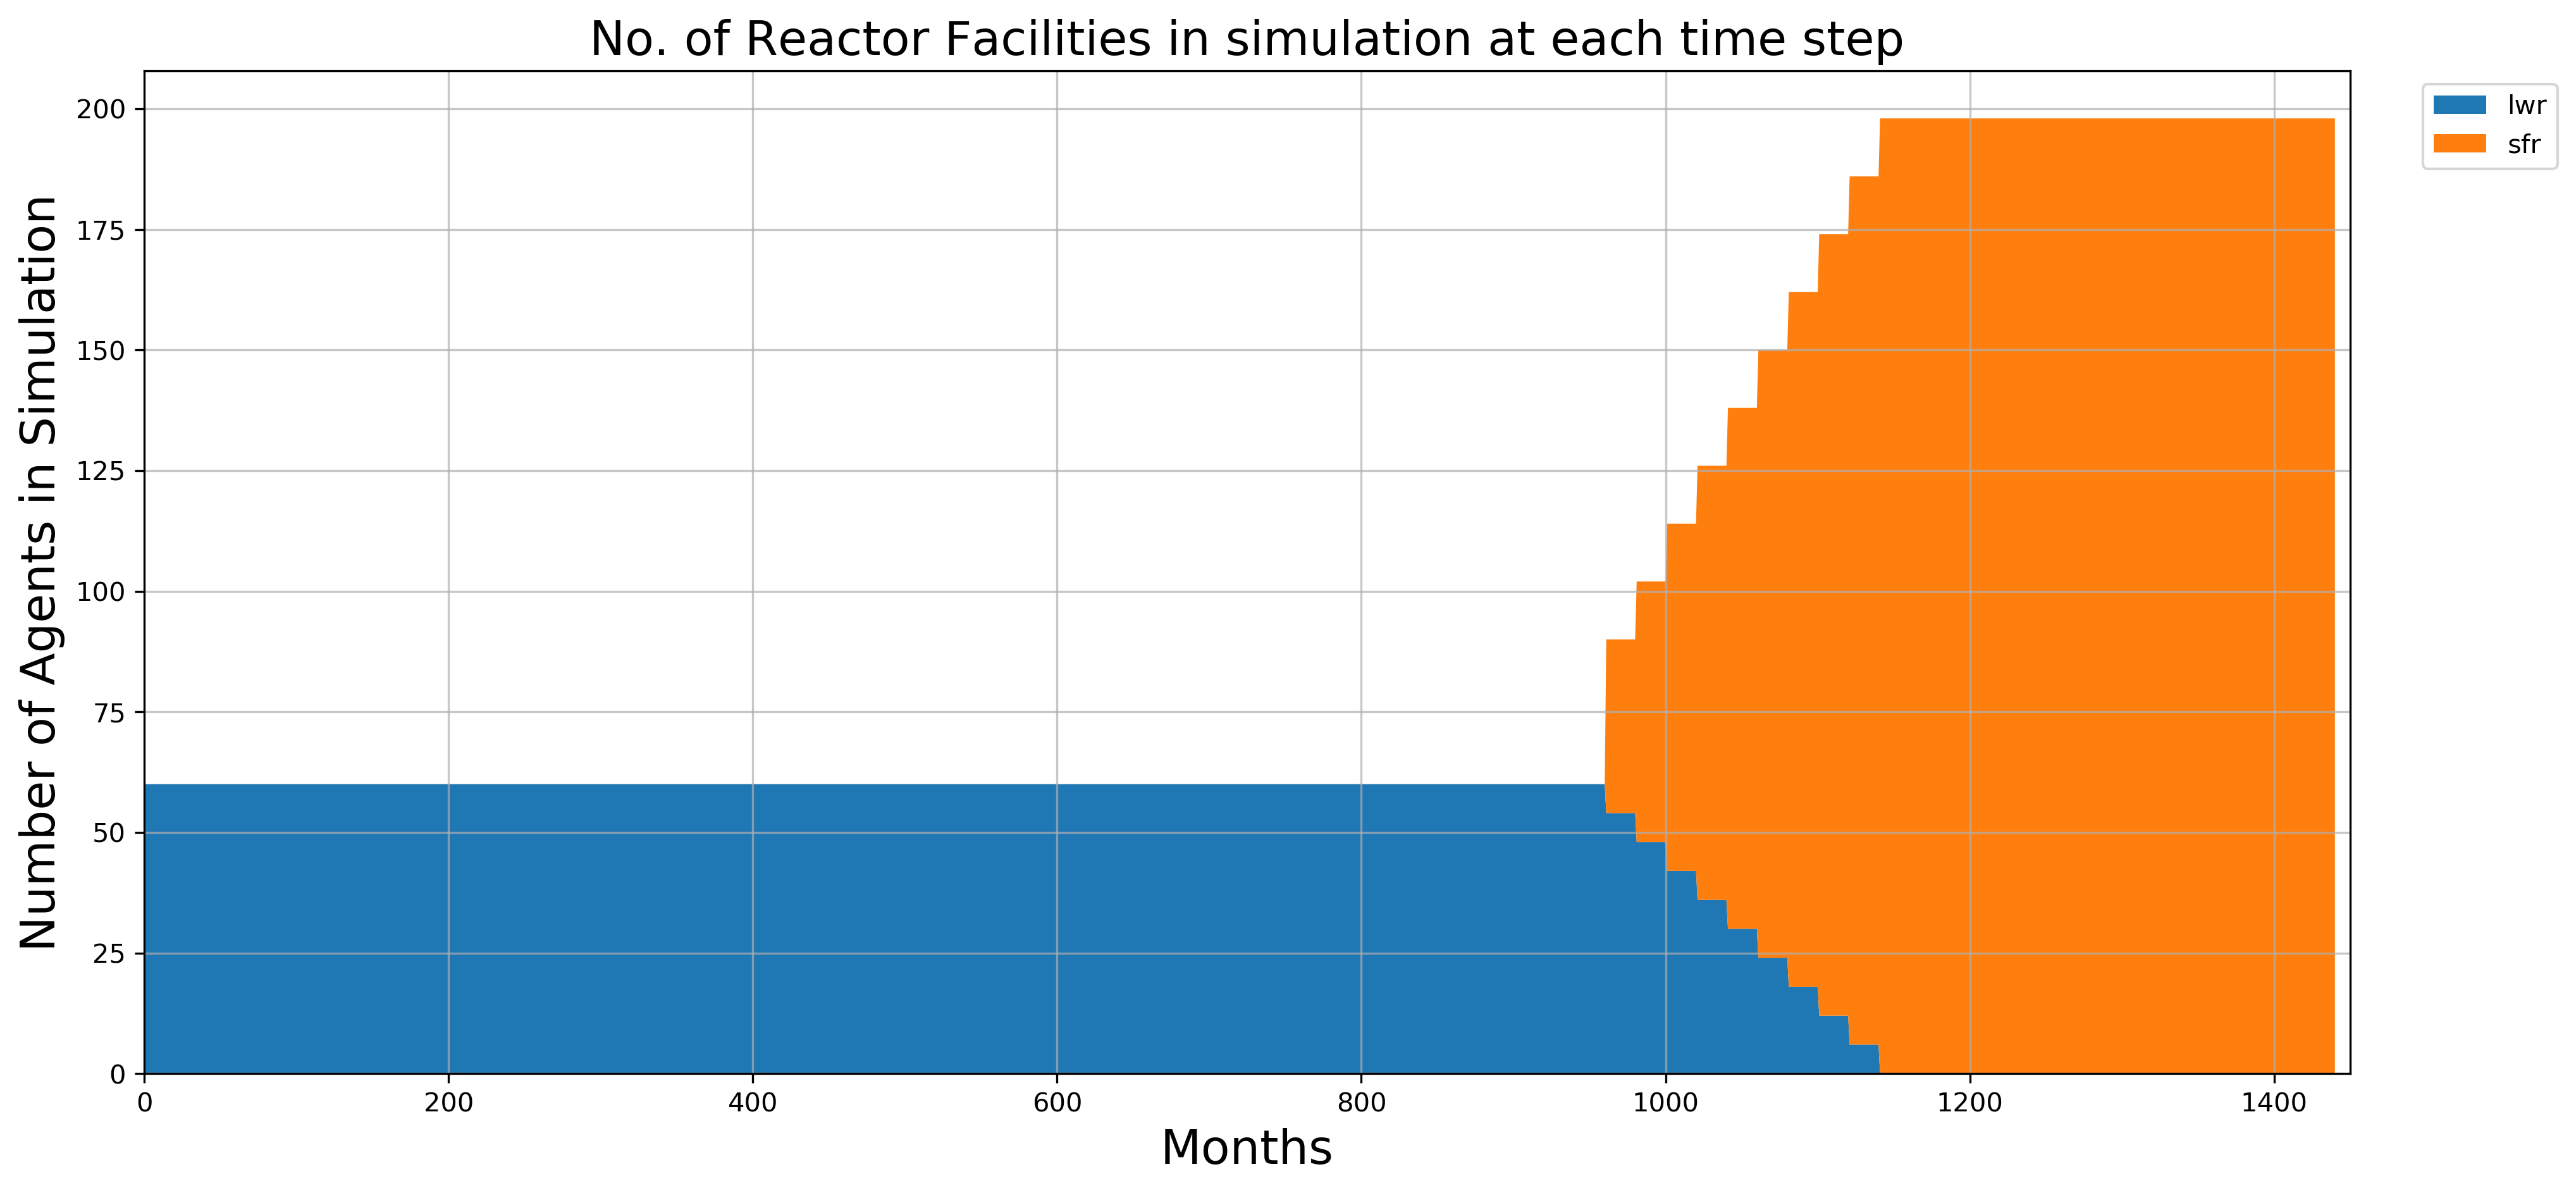
\includegraphics[width=\textwidth]{../paper/figures/eg23-stack_reactor.png}
        \end{center}
              \caption{Time dependent deployment of reactor facilities in 
              the EG01-23 constant power demand transition scenario. 
              \deploy automatically deploys reactor facilities 
              to set up a supply chain to meet constant power demand of $60000$ MW
              during a transition from \glspl{LWR} to \glspl{SFR}}.
      \end{figure}
\end{frame}

\begin{frame}
    \frametitle{Best Performing Transition Scenarios}
    \textbf{EG01-23: Constant Power Demand}
    \begin{figure}[htbp!]
        \begin{center}
          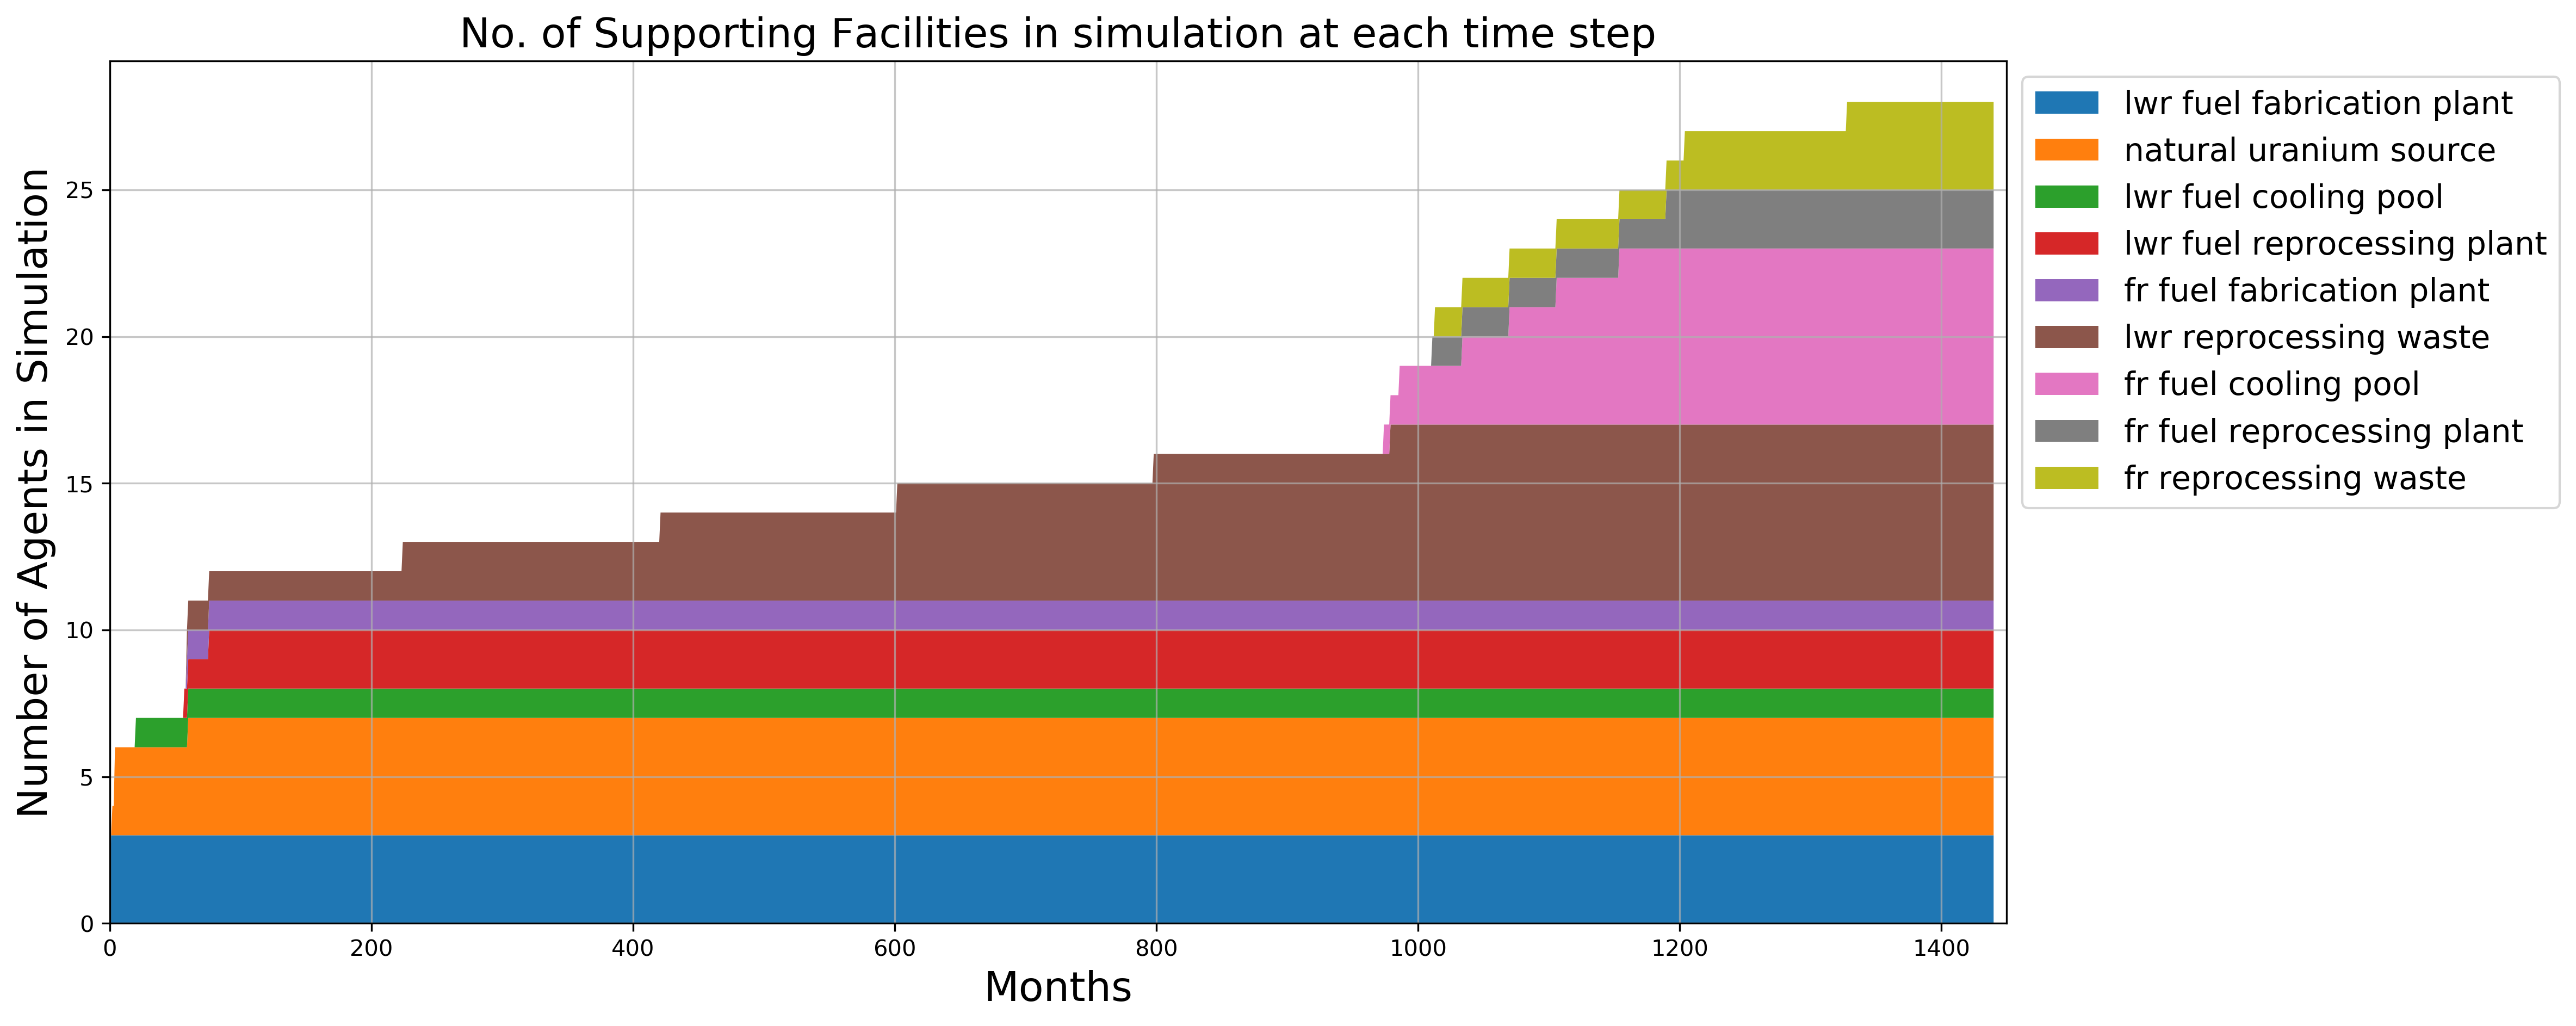
\includegraphics[width=\textwidth]{../paper/figures/eg23-stack_support.png}
        \end{center}
              \caption{Time dependent deployment of supporting facilities in 
              the EG01-23 constant power demand transition scenario. 
              \deploy automatically deploys reactor facilities 
              to set up a supply chain to meet constant power demand of $60000$ MW
              during a transition from \glspl{LWR} to \glspl{SFR}}.
      \end{figure}
\end{frame}

\begin{frame}
    \frametitle{Best Performing Transition Scenarios}
    \textbf{EG01-30: Linearly Increasing Power Demand}
    \begin{figure}[htbp!]
        \begin{center}
          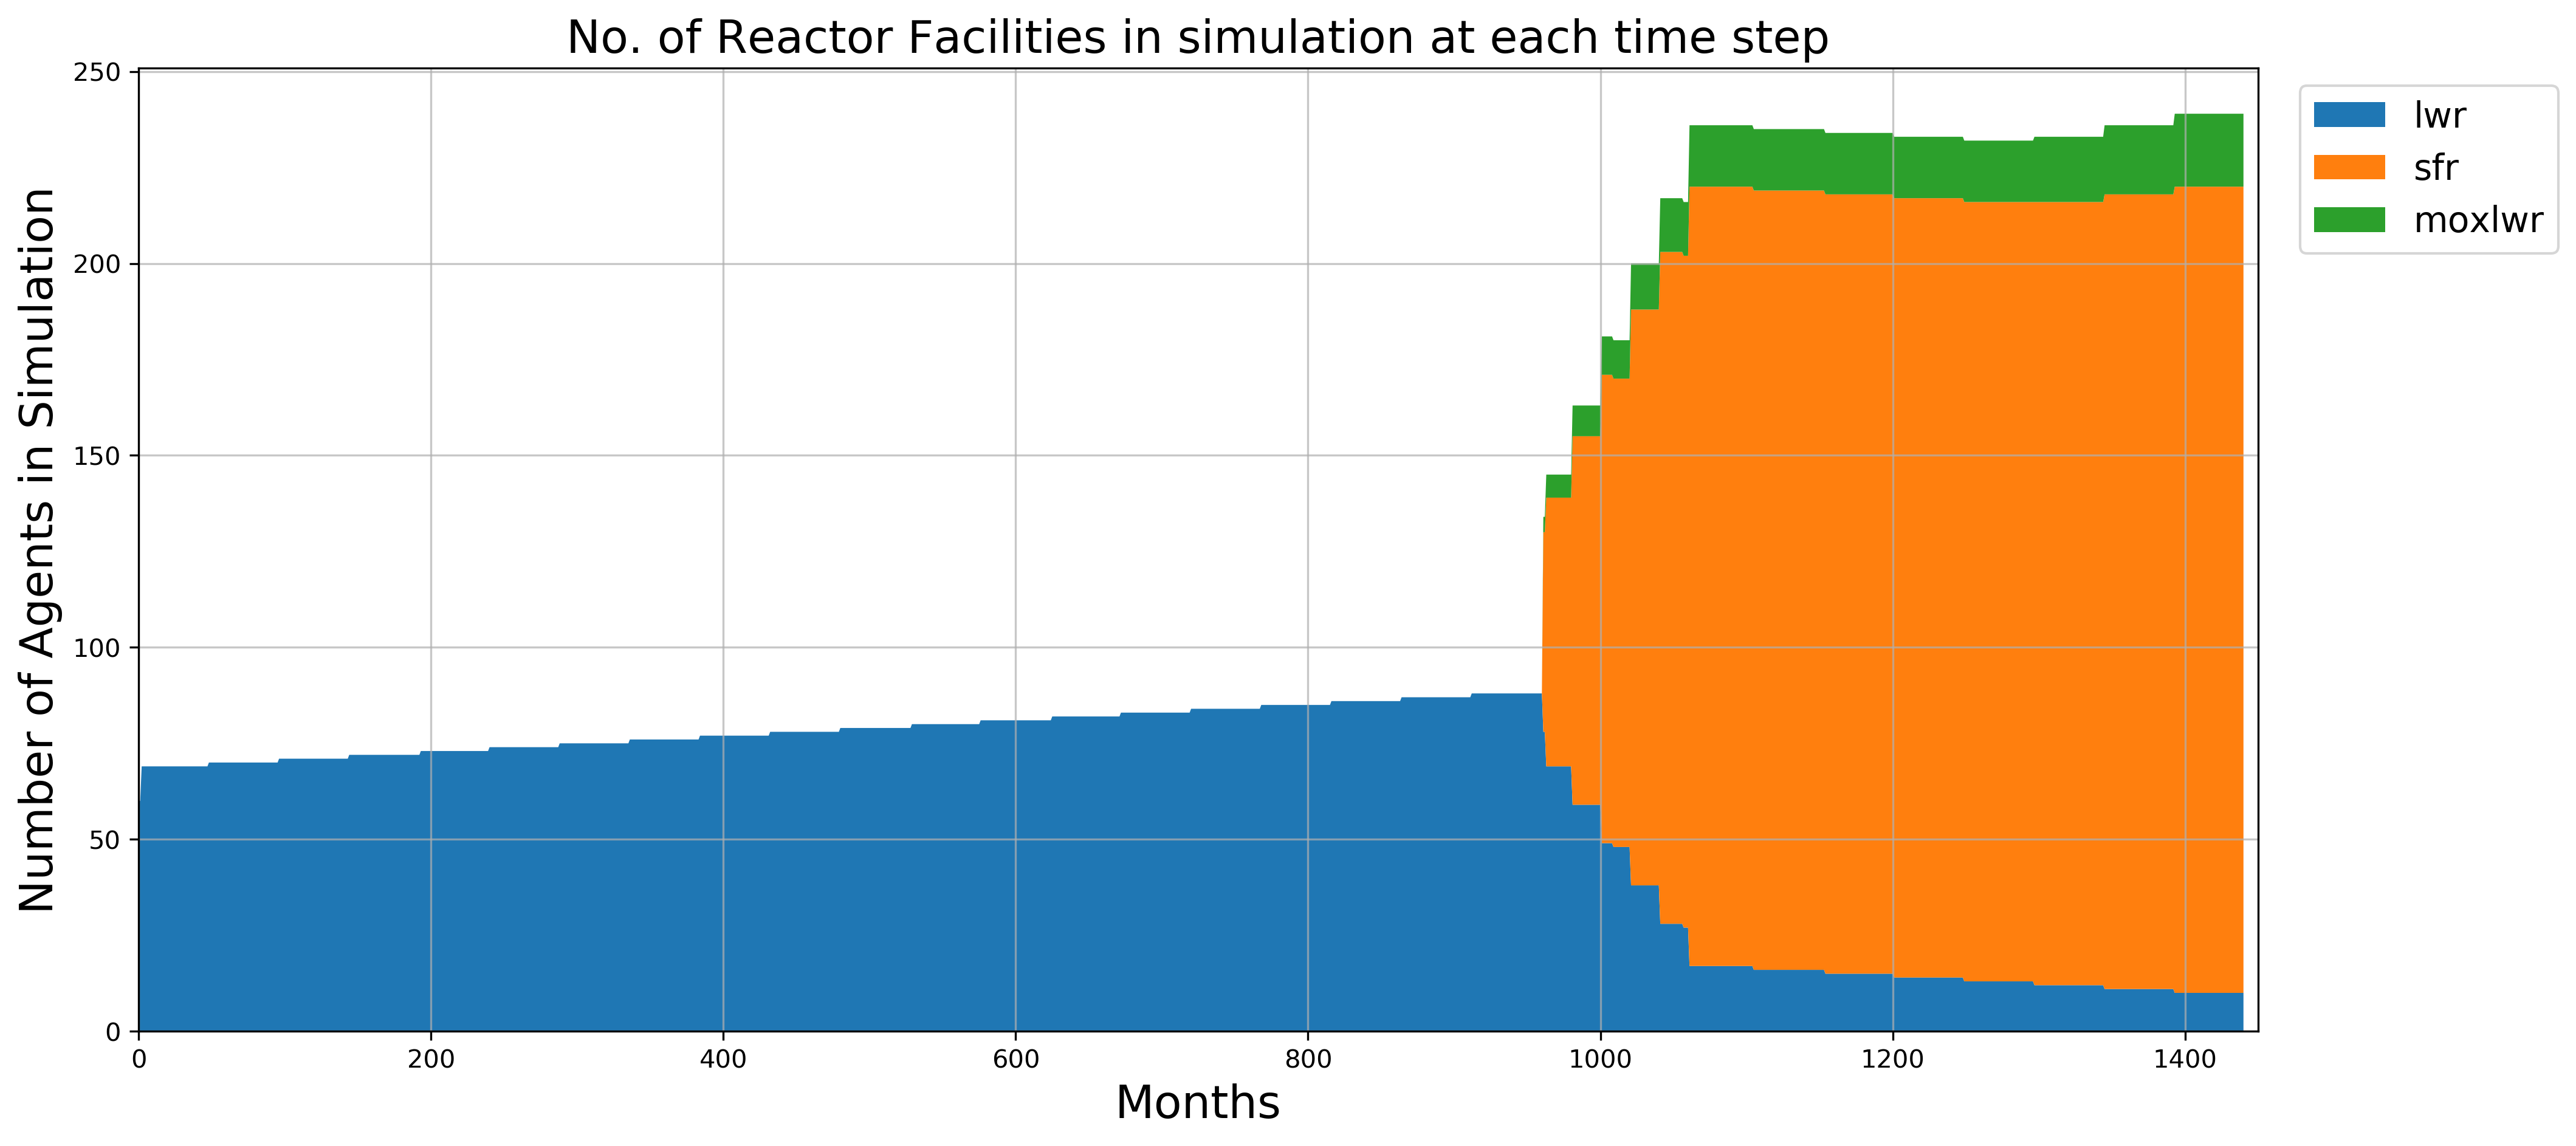
\includegraphics[width=\textwidth]{../paper/figures/eg30-stack_reactor.png}
        \end{center}
              \caption{Time dependent deployment of reactor facilities in 
              the EG01-30 linearly increasing power demand transition scenario. 
              \deploy automatically deploys reactor facilities 
              to set up a supply chain to meet constant power demand of $60000+250t/12$ MW
              during a transition from \glspl{LWR} to \glspl{SFR}}.
      \end{figure}
\end{frame}

\begin{frame}
    \frametitle{Best Performing Transition Scenarios}
    \textbf{EG01-30: Linearly Increasing Power Demand}
    \begin{figure}[htbp!]
        \begin{center}
          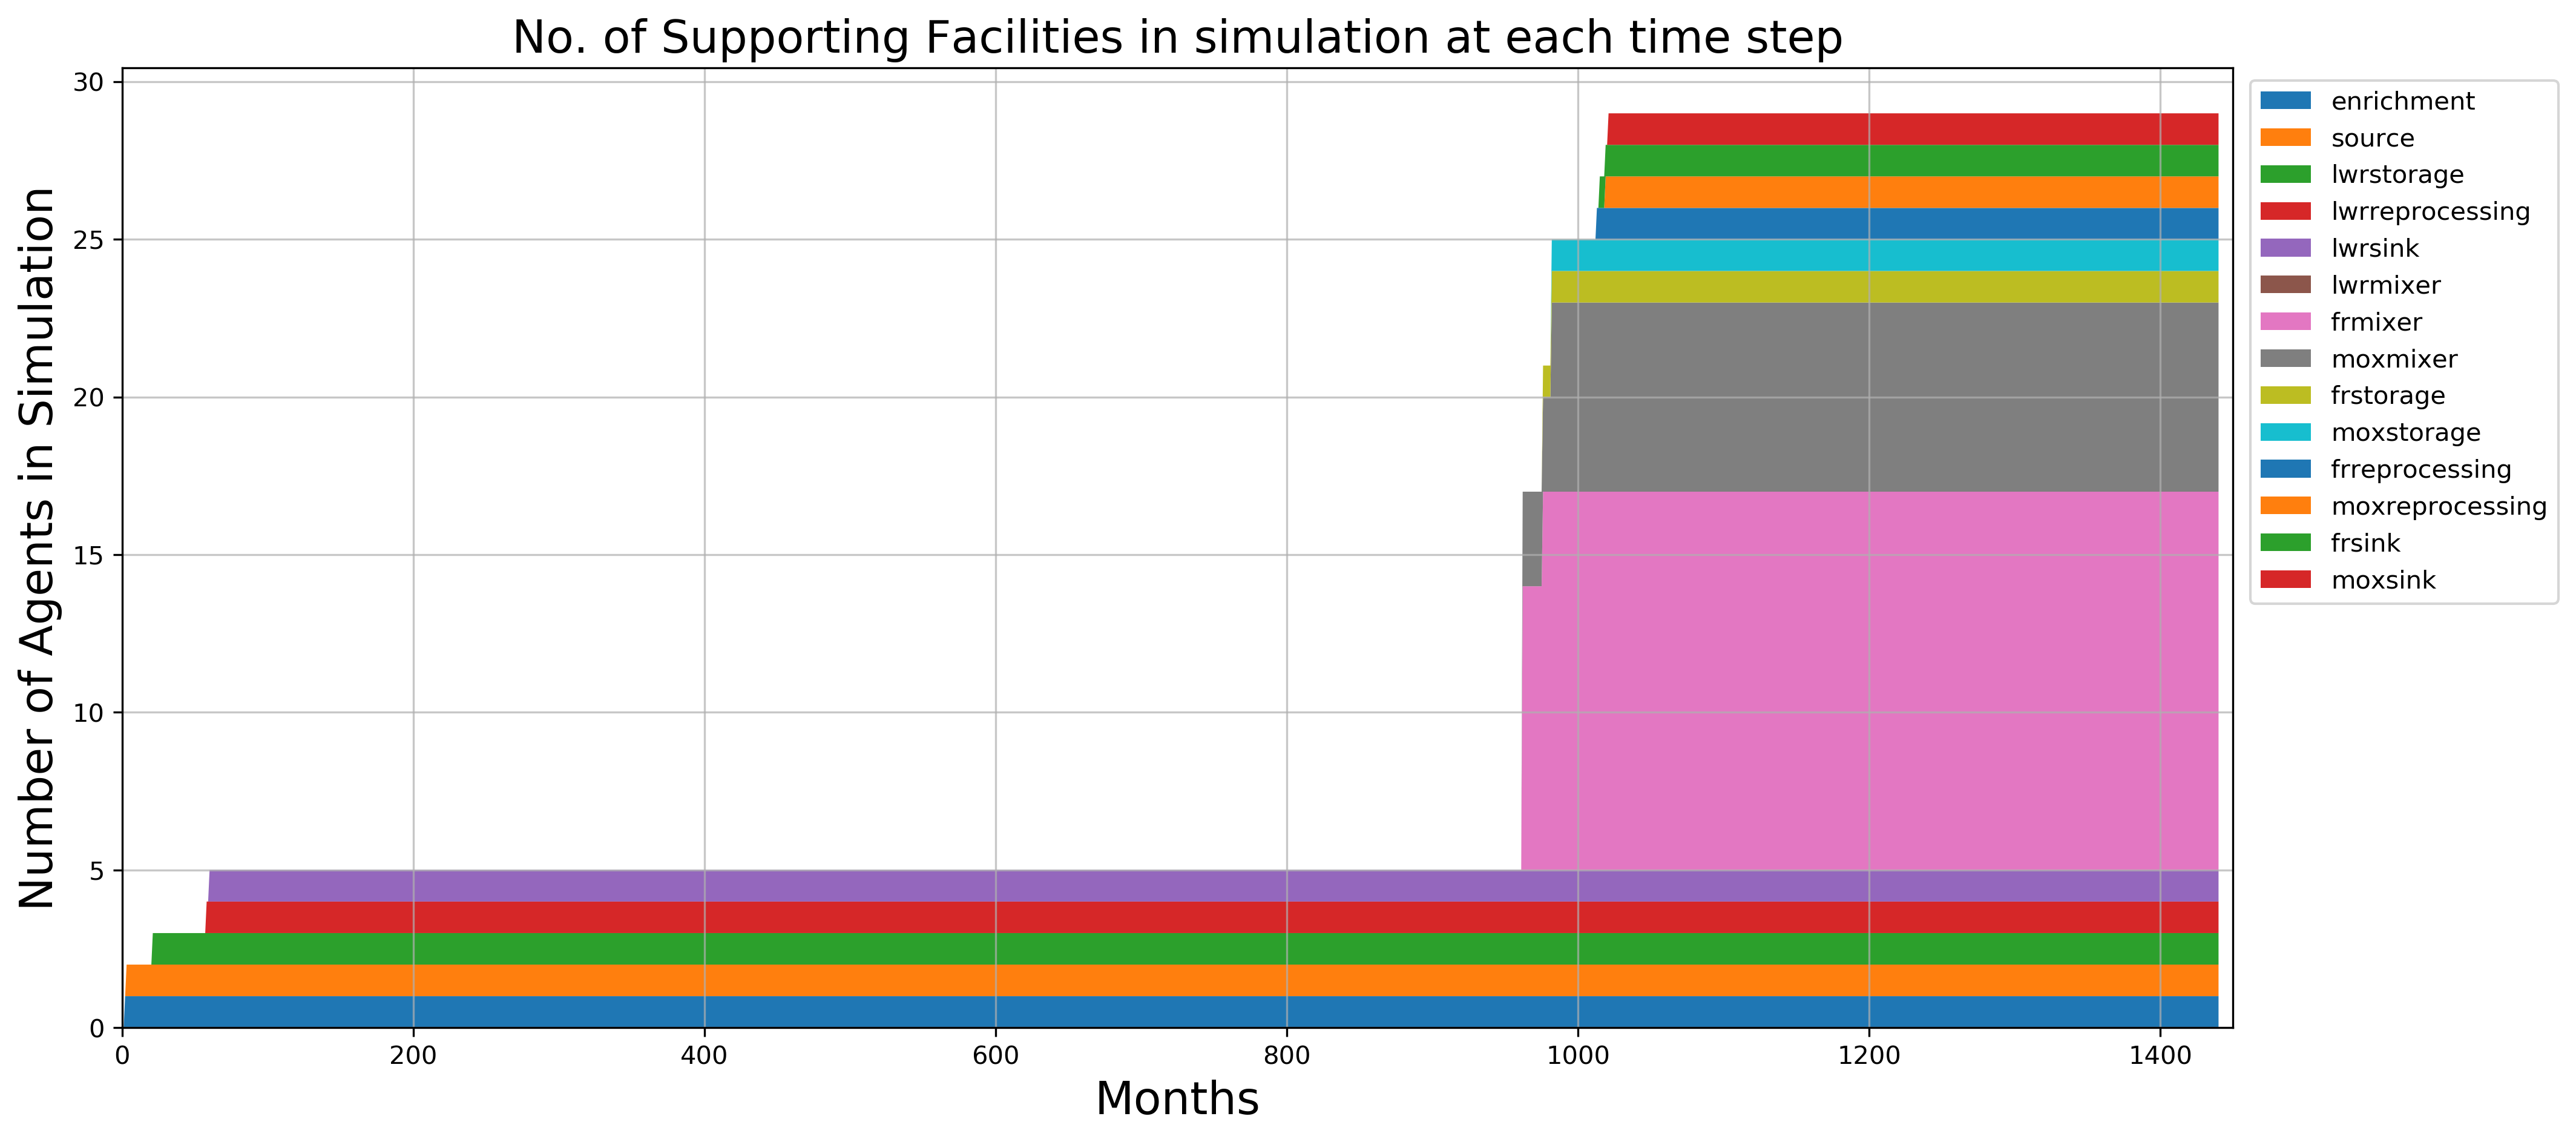
\includegraphics[width=\textwidth]{../paper/figures/eg30-stack_support.png}
        \end{center}
              \caption{Time dependent deployment of supporting facilities in 
              the EG01-30 linearly increasing power demand transition scenario. 
              \deploy automatically deploys reactor facilities 
              to set up a supply chain to meet constant power demand of $60000+250t/12$ MW
              during a transition from \glspl{LWR} to \glspl{SFR}}.
      \end{figure}
\end{frame}

\begin{frame}
    \frametitle{Best Performing Transition Scenarios}
    \textbf{Undersupply and under capacity of commodities for the best performing transition scenarios} 
    \begin{table}[]
        \centering
            \caption{Undersupply/capacity of commodities for the best performing EG01-EG23,24,29,30 transition scenarios.}
            \label{tab:all-power}
            \footnotesize
            \begin{tabularx}{\textwidth}{l|RRRR}
            \hline
            & \multicolumn{3}{|c}{\textbf{Undersupplied Time Steps}} \\ \hline
            \textbf{Transition Scenario} & EG01-EG23 & 
            EG01-EG24 & EG01-EG29 & 
            EG01-EG30 \\ 
            \textbf{Power Demand} &Constant&Linearly Increasing&Constant&Linearly Increasing \\
            \textbf{Prediction Method} &\texttt{poly}&\texttt{fft}&\texttt{poly}& \texttt{fft}\\
            \textbf{Power Supply Buffer [MW]} &0&6000&0&8000 \\ \hline
            \textbf{Commodities} \\ 
            Natural Uranium		    & 2 	& 3  &  1  & 1 \\ 
            \gls{LWR} Fuel     	    & 4 	& 6  &  1  & 2\\ 
            \gls{SFR} Fuel     	    &  0 	& 0  &  2  & 2\\ 
            \gls{MOX} \gls{LWR} Fuel &-&-&2&2 \\
            Power      				&  6 	& 7  &  4 &  5\\ 
            \gls{LWR} Spent Fuel	& 1 	& 1  & 1 & 1\\ 
            \gls{SFR} Spent Fuel     	    &  1 	& 1  &  1  & 1\\ 
            \gls{MOX} \gls{LWR} Spent Fuel &-&-&1&1 \\ \hline 
        \end{tabularx}
    \end{table}
    
\end{frame}